\chapter{Introduction}
\label{chap:intro}

% \begin{figure}[H]
%     \centering
%     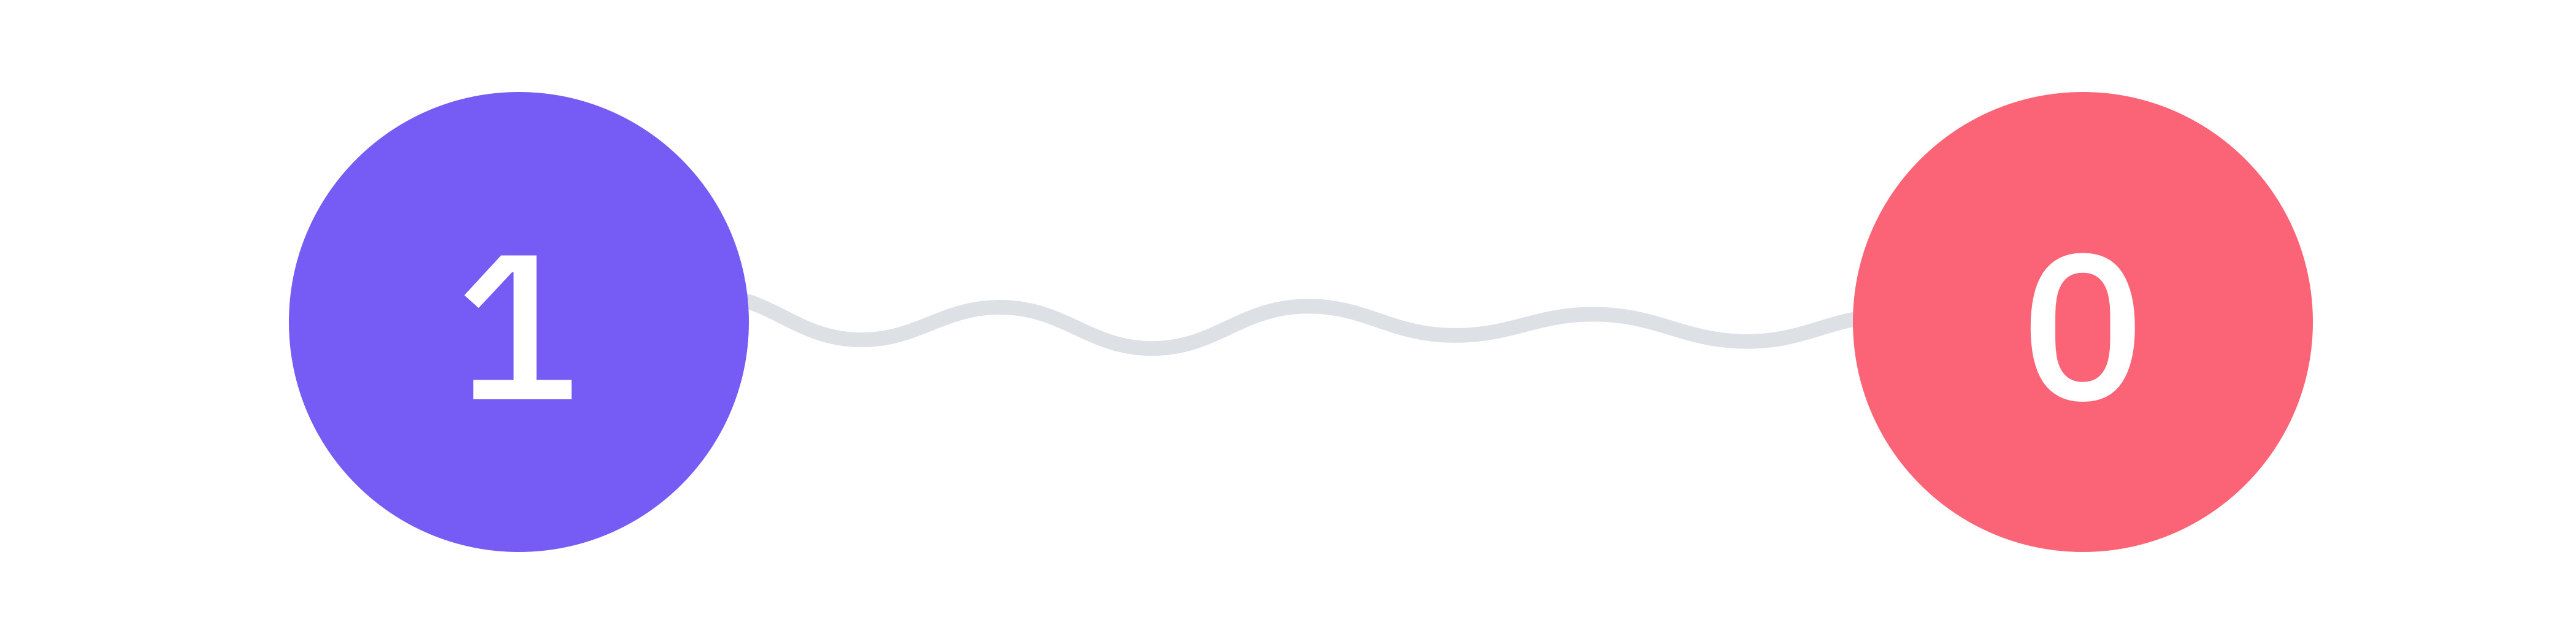
\includegraphics[alt={Testo alternativo dell'immagine}, width=1\columnwidth]{img/quantum_entanglement.jpeg}
%     \caption{Lorem}
%     \label{fig:entanglement}
% \end{figure}
% 
% Introduzione al contesto applicativo.
% 
% Lorem Figure \ref{fig:entanglement}
% 
% Esempio di utilizzo di un termine nel glossario \gls{api}.
% 
% Esempio di citazione direttamente nel testo \cite{site:agile-manifesto}.
% 
% Esempio di citazione nel piè di pagina \footcite{womak:lean-thinking}.
% Introduzione all'idea dello stage\footcite{article:spooky}.

\section{Mobile accessibility: context \& foundations}
\label{chap:intro-background}

In an era where digital technology permeates every aspect of our lives, mobile devices have emerged as the primary gateway to the digital world, allowing a lot of new people to be connected at any given time, no matter the condition. An estimated number of circa 7 billions \cite{article:number-of-users}, representing a dramatic increase from just one billion users in 2013. This explosive growth has not only changed how we communicate and access information but has also created a massive market for different needs and introduced new categories of users, with different habits and cultures into a truly global market.

As mobile applications become increasingly central to daily life, ensuring their accessibility to all users, regardless of their abilities or disabilities, has become a critical imperative, since not only technology should be able to connect, but also to unite seamlessly people with different capabilities. Accessibility refers to the design and development practices enabling all users, regardless of their abilities or disabilities, to perceive, understand and navigate with digital content effectively. Not only the quantity of media increased, but also the quantity of different media which allow to access information definitely increased; finding appropriate measurements to establish a good level of understanding and usability is important and finding appropriate levels of measurements is non-trivial. \\

An estimated portion of over one billion people lives globally with some forms of disability \cite{article:who-disability}. Inaccessible mobile applications can, therefore, present considerable barriers to participation in that large and growing part of modern life that involves education, employment, social interaction, and even basic services. Accessibility is not about a majority giving special dispensation to a minority but rather about providing equal access and opportunities to very big and diverse user bases.

This encompasses a wide range of considerations to be made on the actual products design and the user classes, including but not limited to:
\begin{enumerate}
    \item \textit{Visual accessibility}: supporting users who are blind or have low vision, requiring alternative description, a clear language and screen readers support;

    \item \textit{Auditory accessibility}: providing alternatives for users who are deaf or hard of hearing, offering clear controls and alternative  visuals for audio content, ensuring compatibility with assistive devices and giving feedback to specific actions done by users;

    \item \textit{Motor accessibility}: accommodating users with limited dexterity or mobility, providing alternative input navigation, create a design so to help avoiding complex gestures, customize the interactions and gestures, reducing precision and accommodating errors;

    \item \textit{Cognitive accessibility}: ensuring content is understandable for users with different cognitive abilities, creating a consistent and predictable navigation, visual support on UI so to support focus and attention and enhancing comprehension of interface components.
    
\end{enumerate}

These considerations are important since they impact how accessibility features should go above and beyond, carefully considering the design in terms of \gls{uig} (\acrshort{ui}), considering the design and layout of interactive elements and the actual experience in using the product, considering the degree of satisfaction and meeting of user's needs, so the \gls{uxg} (\acrshort{ux}).  

In the mobile environment, such considerations is important, since there is a complex web of interactions to be considered, mainly focusing on two aspects:

\begin{enumerate}
    \item Device diversity and integration - accommodating different gestures, interfaces and interaction modalities
        \begin{itemize}
            \item Traditional mobile devices (smartphones, tablets)
            \item Emerging form factors (foldables, dual-screen devices)
            \item Wearable technology (smartwatches, fitness trackers)
            \item Embedded systems (vehicle interfaces, smart home controls)
            \item IoT devices with mobile interfaces
        \end{itemize}
    \item Usage context variations - may influence the overload of information and the cognitive load perceived by the user
        \begin{itemize}
            \item Environmental conditions (lighting, noise, movement)
            \item User posture and mobility situations
            \item Attention availability and cognitive load
            \item Physical constraints and limitations
            \item Social and cultural contexts
        \end{itemize}
\end{enumerate}

These considerations are important since they impact how accessibility features should go above and beyond, carefully considering how the interaction in mobile devices is used. Mobile devices offer multiple interaction modalities, which must be considered for an inclusive design:

\begin{itemize}
    \item \textit{Touch-based interactions}: here, traditional interactions present specific challenges and opportunities for accessibility: actions like tapping (selection/activation), double tapping (confirmation/secondary actions), long pressing (contextual menus/additional options), swiping (navigation/list scrolling) and pinching (zoom control) are used. These gestures may need alternatives regarding timing in long presses, touch stabilization and increased touch target sizes, since they can be also combined with multiple patterns e.g. multi-finger gestures and edge swipes;
    \item \textit{Voice control and speech input}: navigation commands and action triggers can be activated giving directions (e.g. "go back", "scroll down"), inputting text thorough dictation, while giving auditory feedback and interactions vocally;
    \item \textit{Motion and sensor-based input}: modern devices offer various sensor-based interaction methods, like tilting controls for navigation, shaking gestures for specific actions, orientation changes for layout adaptation, using proximity sensors to detect gestures without touch;
    \item \textit{Switch access and external devices}: providing support for alternative input methods is crucial, providing physical single or multiple switch support, sequential focus navigation and customizable timing controls. Some users might find useful to have external input devices like keyboards, specialized controllers, Braille displays, but also help from custom assistive devices;
    \item \textit{Haptic feedback}: tactile feedback provides important interaction cues, on actions confirmation, error notifications and context-sensitive responses, e.g. force-touch interactions and pressure-based controls.
\end{itemize}

It's useful to analyze such commands since the focus would be describing how to address accessibility issues and have a complete focus on how a user would interact with an interface and a mobile device, since each interaction provides a different degree of complexity. Understanding built-in capabilities is crucial for developers working with cross-platform frameworks, as they must effectively bridge their applications with native features. These tools will be discussed from an high-level, so to describe their role and goals, among functionalities:

\begin{itemize}
    \item \textit{TalkBack for Android}: Google's screen reader provides comprehensive accessibility support through:
        \begin{itemize}
            \item Touch exploration mode allowing users to hear screen content by touching it
            \item Custom gesture navigation system for efficient interface interaction
            \item Customizable feedback settings for different user preferences
            \item Integration with external Braille displays and keyboards (also with complementary services like \textit{BrailleBack})
            \item Support for different languages and speech rates
            \item Help in combination of \textit{Switch Access}, built-in feature to help users using switches instead of touch gestures
        \end{itemize}
    
    \item \textit{VoiceOver for iOS}: Apple's integrated screen reader offers:
        \begin{itemize}
            \item Rotor control for customizable navigation options
            \item Advanced gesture recognition system
            \item Direct touch exploration of screen elements
            \item Automatic language detection and switching
            \item Comprehensive Braille support across multiple standards
            \item Complete integration with \textit{Zoom}, a built-in screen magnifier present in iOS devices to zoom in on any part of the screen
            \item Integrated with other a suite of other accessibility tools present in iOS devices, available to all users
        \end{itemize}

    \item \textit{Select to Speak for Android}: A complementary feature that provides:
        \begin{itemize}
            \item On-demand reading of selected screen content
            \item Visual highlighting of spoken text
            \item Simple activation through dedicated gestures
            \item Integration with system-wide accessibility settings
        \end{itemize}
\end{itemize}

In the thesis, apart from considering the degree of importance of each kind of interactions, the implementation of accessibility support between two of the most popular mobile development frameworks will be given. The implementation of accessibility support varies significantly between Flutter and React Native, particularly in how they interact with these native features. Flutter creates an accessibility tree that maps to native accessibility APIs, while React Native provides direct bindings to platform-specific accessibility features. This fundamental difference affects how developers must approach accessibility implementation in their applications and such will be explored in related chapters and subsections.

\section{Related works}
\label{chap:intro-related-works}

Research in mobile accessibility spans multiple areas, from user interaction studies to framework-specific analyses. This section presents relevant work organized by key research themes that inform our framework comparison approach. Different studies will be presented here, discussing the importance of studies between people and interaction with mobile devices, may they be with disabilities or not, evaluating accessibility barriers and understanding guidelines which can be generally used. \\

Lian et al. \cite{lian2021autism} explored the usability of augmented reality (AR) applications for children with autism. By employing eye-tracking technology, the interaction patterns of children were studied upon the usage of coloring, revealing children with autism have distinct gaze patterns compared to neurotypical children, often focusing on certain UI elements. This underscores the importance of designing interfaces for users with cognitive disabilities, ensuring they are intuitive enough to be understood under all circumstances.

\section{Thesis structure}
\label{chap:intro-structure} 

In this subsection, a brief description of the rest of the thesis is given:

\begin{description}
    \item[{\hyperref[chap:accessibility]{The second chapter}}]  examines accessibility guidelines specific to mobile applications, including WCAG mobile adaptations, platform-specific requirements for iOS and Android, legal framework regulations, implementation considerations and testing methodologies;
    
    \item[{\hyperref[chap:frameworks]{The third chapter}}] provides an overview of Flutter and React Native architecture and component modeling, while discussing framework-specific accessibility support features;
    
    \item[{\hyperref[chap:implementation]{The fourth chapter}}] describes precisely the implementation of the WCAG guidelines, providing implementation complexity, performance implications, developer experience, testing approaches, while discussing best practices and finding limitations;
    
    \item[{\hyperref[chap:conclusions]{The last chapter}}] summarizes finding and provides recommendations, best practices for accessible development and future research directions.
\end{description}

Regarding the text composition, the following typographical conventions have been adopted for this document:
\begin{itemize}
    \item Acronyms, abbreviations, and technical terms are defined in the glossary;
    \item First occurrences of glossary terms use the format: \gls{uig};
    \item Foreign language terms and technical jargon appear in \textit{italic};
    \item Code examples use \texttt{monospace} formatting when discussed within text or proper custom coloring form to be used within the rest of sections.
\end{itemize}

\newpage